
\documentclass[12pt]{article}

\usepackage[utf8]{inputenc}
\usepackage[greek, english]{babel}

% Packages
\usepackage{alphabeta}
\usepackage{amsmath}
\usepackage{amsthm}
\usepackage{caption}
\usepackage{color}
\usepackage{float}
\usepackage{fullpage}
\usepackage{graphicx}
\usepackage{hyperref}
\usepackage{latexsym}
\usepackage{listings}
\usepackage{pxfonts}
\usepackage{stackrel}
\usepackage{subfig}
\usepackage{tikz}
\usepackage{titlesec}

% Commands
\newcommand{\N}{\mathbb{N}}
\newcommand{\R}{\mathbb{R}}
\newcommand{\abs}[1]{\left\lvert#1\right\rvert}
\newcommand{\code}[2]{\lstinputlisting[caption={#2}]{#1}}
\newcommand{\margin}{\hspace{4pt}}
\newcommand{\norm}[1]{\left\lVert#1\right\rVert}

% Environments
\newenvironment{matlab}
	{\begin{figure}[H]\centering\captionsetup{justification=centering}}
	{\end{figure}}

\newenvironment{rcases}
	{\left.\begin{aligned}}
	{\end{aligned}\right\rbrace}

% Python Syntax Highlighting
\definecolor{string_color}{RGB}{0, 161, 13}
\definecolor{comment_color}{RGB}{46, 46, 46}
\definecolor{keyword_color}{RGB}{0, 112, 191}
\definecolor{background_color}{RGB}{250, 250, 250}

\lstset{
    framesep=15pt,
    xleftmargin=15pt,
    xrightmargin=15pt,
    language=Python,
    captionpos=b,
    numbers=right,
    numberstyle=\small\ttfamily,
    frame=lines,
    showspaces=false,
    showtabs=false,
    breaklines=true,
    showstringspaces=false,
    breakatwhitespace=true,
    commentstyle=\color{comment_color}\textit,
    keywordstyle=\bfseries\color{keyword_color}\textbf,
    stringstyle=\color{string_color}\textit,
    morekeywords={self, lambda, __init__, __del__, __name__, for, in, not, and, or, :},
    basicstyle=\small\ttfamily,
    tabsize=4,
    keepspaces=true,
    columns=flexible,
    backgroundcolor=\color{background_color}
}

% Links
\hypersetup{
    colorlinks=true,
    linkcolor=blue,
    filecolor=magenta,
    urlcolor=cyan,
}

% Lengths
\setlength{\parindent}{0in}
\setlength{\oddsidemargin}{0in}
\setlength{\textwidth}{6.5in}
\setlength{\textheight}{10in}
\setlength{\topmargin}{-1.0in}
\setlength{\headheight}{18pt}

\titlespacing*{\subsection}
{0pt}{5.5ex plus 1ex minus .2ex}{4.3ex plus .2ex}

\title{\hugeΥπολογιστική Γεωμετρία\\Πρώτη Εργασία}
\author{Σιώρος Βασίλειος - 1115201500144\\Ανδρινοπούλου Χριστίνα - 1115201500006}
\date{Μάρτιος 2020}

\begin{document}

\maketitle

\pagenumbering{gobble}

\pagebreak


\subsection*{1. Implement an algorithm that takes as input three points in the plane. checks
that they form a triangle and whether the interior of the triangle contains the origin (0, 0) or
not.}

\pagebreak

\subsection*{2. Given a circle of radius r in the plane with (0, 0) as center, implement an
algorithm that finds the total lattice points on the circumference. Lattice Points are points
with integer coordinates.}

\subsubsection*{Thought Process}

Σε ένα καρτεσιανό σύστημα συντεταγμένων, ένας κύκλος με κέντρο το σημείο (a, b)
και ακτίνα r είναι ένα σχήμα το οποίο αποτελείται από όλα τα σημεία των οποίων
οι συντεταγμένες ικανοποιούν την εξίσωση \\

\[ (x - a) ^ 2 + (y - b) ^ 2 = r ^ 2 \]

Από την παρπάνω εξίσωση, μπορούμε να συμπεράνουμε,
ότι οποιοδήποτε σημείο, του οποίου η Ευκλείδια απόσταση από το κέντρο του κύκλου
είναι μεγαλύτερη της ακτίνας του, βρίσκεται εκτός του κύκλου. \\

Αν ο κύκλος έχει ως κέντρο την αρχή των αξόνων, δηλαδή το σημείο \( (0, 0) \), τότε
η παραπάνω εξίσωση παίρνει την εξής απλούστερη μορφή \\

\[ x ^ 2 + y ^ 2 = r ^ 2 \]

Σε αυτή την περίπτωση, είτε η τετμημένη είτε η τεταγμένη ενός σημείου
αρκεί να είναι μεγαλύτερη της ακτίνας του έτσι ώστε να μην ανήκει στον κύκλο. \\

Ως εκ τούτου, τα σημεία πλέγματος ενός κύκλου ακτίνας r με κέντρο το (0, 0)
είναι υποσύνολο του συνόλου που απαρτίζεται από σημεία με ακέραιες συνταγμένες
στο εύρος \( [-r, +r] \) και στις δύο διαστάσεις, με την πρόσθετη συνθήκη
να ικανοποιούν την παραπάνω εξίσωση έτσι ώστε να βρίσκονται επί της
περιφέρειάς του. \\

Για παράδειγμα, για έναν κύκλο ακτίνας 1 με κέντρο το (0, 0) αρκεί να
ελέγξουμε ποιά από τα σημεία εντός του συνόλου \\

\[ \{ (-1, 0), (0, -1), (0, +1), (+1, 0) \} \]

ικανοποιούν την εξίσωση

\[ x^2 + y^2 = 1 \]

\pagebreak

\subsubsection*{Implementation}

Δεδομένου ότι δεν ήταν ξεκάθαρο, αν το πρόβλημα ζητούσε μόνο
το πλήθος ή και τα ακριβή σημεία πλέγματος,
αποφασίσαμε να ακολουθήσαμε την παρακάτω προσέγγιση η οποία μπορεί να
χρησιμοποιηθεί για την εύρεση και των δύο όπως θα δείτε
στην συνέχεια. \\

\begin{lstlisting}
def lattice_points(radius):
    points = []

    for x in range(-radius, radius + 1):
        for y in range(-radius, radius + 1):
            if x ** 2 + y ** 2 == radius ** 2:
                points.append((x, y))

    return points
\end{lstlisting}

\pagebreak

\subsubsection*{Running the code}

\begin{matlab}
    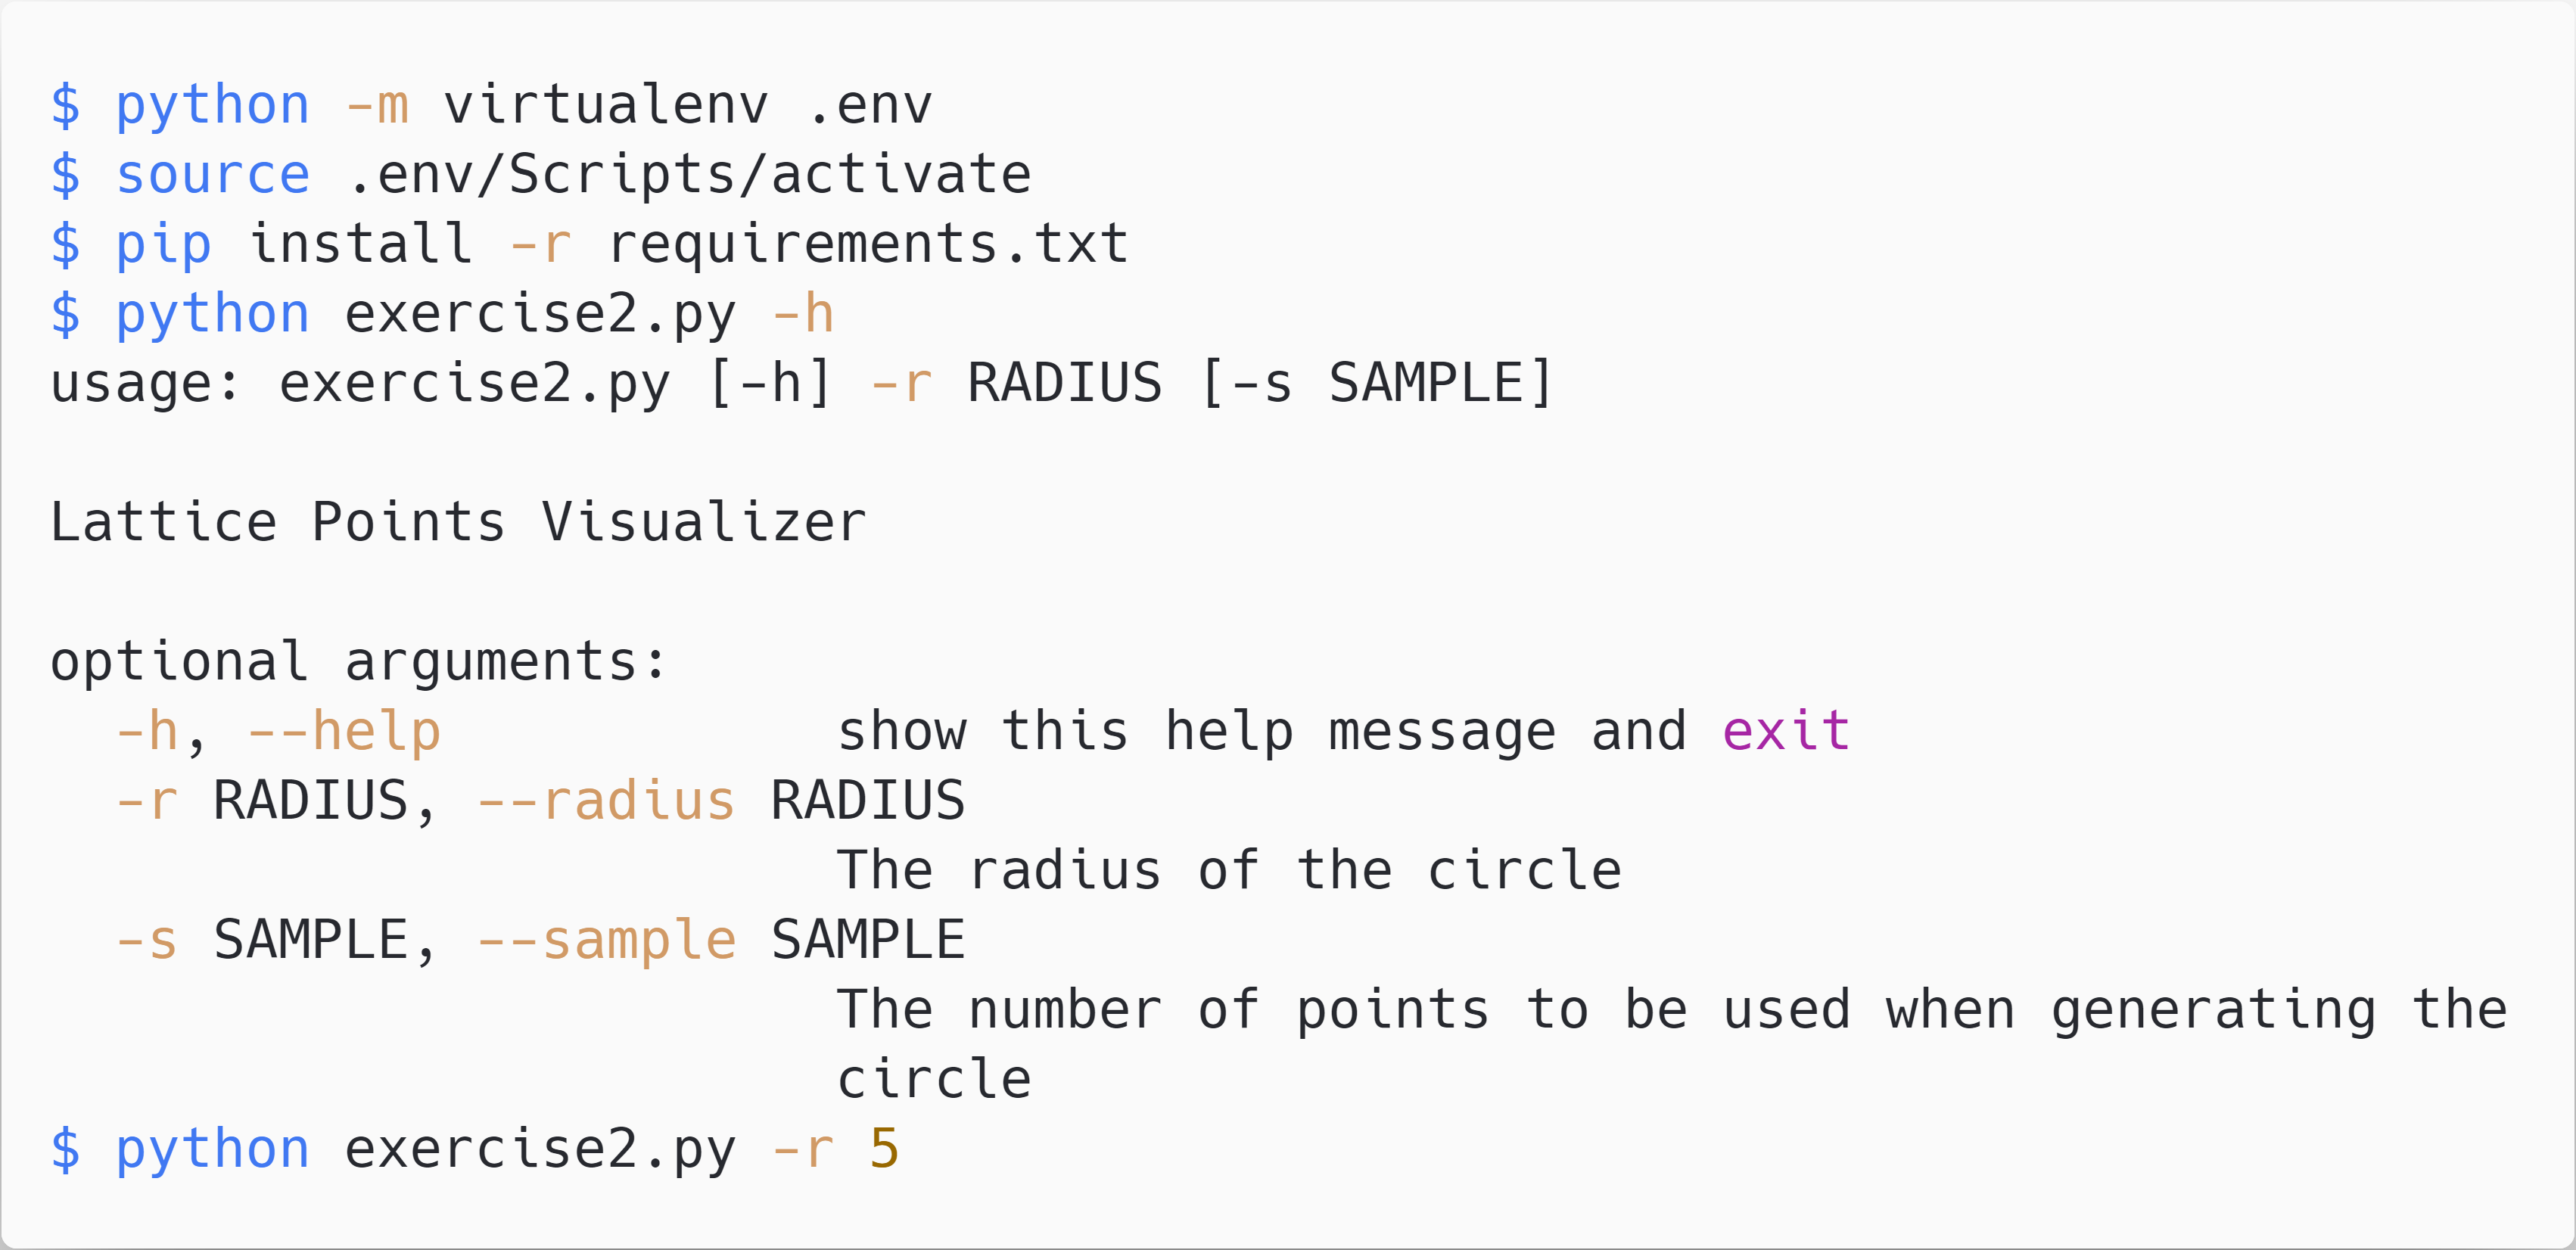
\includegraphics[scale=0.140]{images/lattice_points.png}
\end{matlab}

\subsubsection*{Example Usage}

\begin{matlab}
    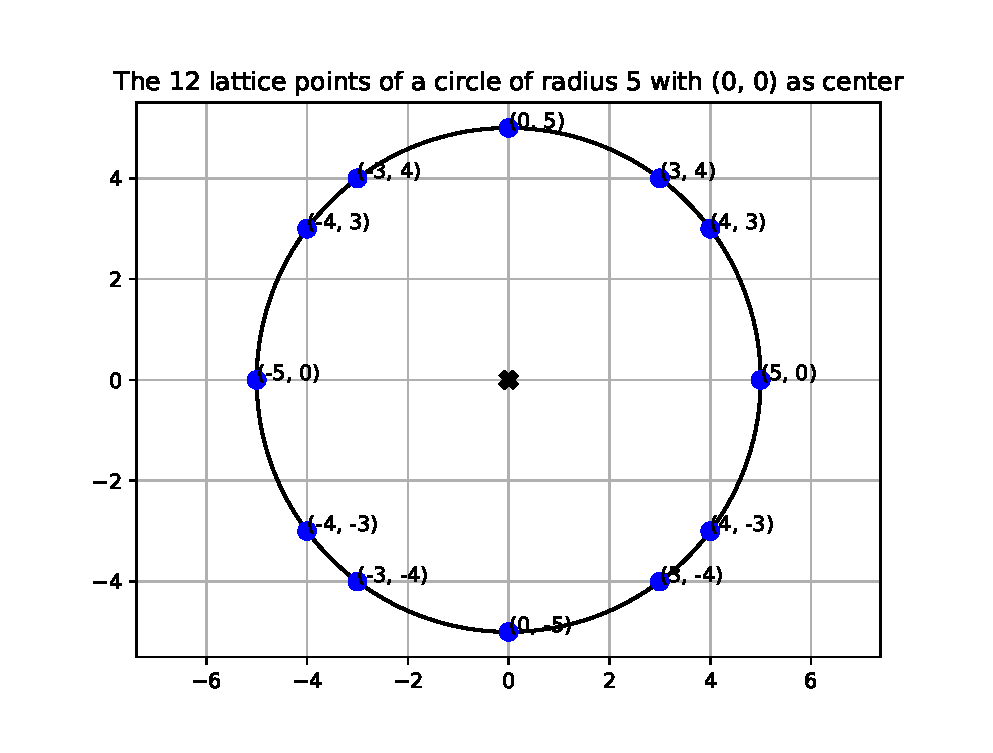
\includegraphics[scale=1]{images/lattice_points.eps}
\end{matlab}

\pagebreak

\subsection*{3. Implement the incremental 2D algorithm for computing the convex hull of a
finite set of points in the plane.}

\pagebreak

\subsection*{4. Implement the gift wrap algorithm for computing the convex hull of a finite
set of points in the plane .}

\subsubsection*{Thought Process}

Ο \textbf{Gift Wrapping} αλγόριθμος, που στην περίπτωση των δύο διαστάσεων είναι
επίσης γνωστός και ως ο \textbf{Jarvis March} αλγόριθμος, μπορεί να περιγραφεί από τα εξής
απλά βήματα \\

\begin{enumerate}
    \item Δεδομένου ενός συνόλου σημείων στον \( \R^2 \),
    επιλέγει ένα σημείο το οποίο είναι γνωστό ότι
    ανήκει στο \textbf{Convex Hull} του συνόλου,
    όπως π.χ. το αριστερότερο σημείο μεταξύ των δεδομένων σημείων.

    \item Στη συνέχεια, επιλέγει ως επόμενο σημείο το σημείο για το οποίο,
    όλα τα υπόλοιπα σημεία βρίσκονται δεξιά της ευθείας που ορίζουν
    το τρέχον και το σημείο αυτό.

    \item Αν το τρέχον σημείο ταυτίζεται με το αρχικά επιλεχθέν σημείο,
    τότε τερμάτησε καθώς το \textbf{Convex Hull} υπολογίστηκε και αποτελείται
    από το σύνολο επιλεχθέντων σημείων έως τώρα. Διαφορετικά επανάλαβε
    το βήμα 2.
\end{enumerate}

\pagebreak

\subsubsection*{Implementation}

Ορίσαμε 3 βοηθητικές συναρτήσεις

\begin{itemize}
    \item \textbf{orientation}: Υπολογίζει τον προσανατολισμο
    των δύο διανυσμάτων που ορίζουν τα 3 σημεία στην είσοδό της

    \item \textbf{counterclockwise}: Με τη βοήθεια της συνάρτηση
    \textbf{orientation} επιστρέφει αν τα τρία αυτά σημεία είναι
    τοποθετημένα με την αντίστροφη φορά του ρολογιού.

    \item \textbf{between}: Με τη βοήθεια της συνάρτηση
    \textbf{orientation} επιστρέφει αν τα τρία αυτά σημεία είναι
    συνευθειακά.
\end{itemize}

\begin{lstlisting}
def orientation(p1, p2, p3):
    return (p3[1] - p1[1]) * (p2[0] - p1[0]) - (p2[1] - p1[1]) * (p3[0] - p1[0])


def counterclockwise(p1, p2, p3):
    return orientation(p1, p2, p3) > 0


def between(p1, p2, p3):
    if orientation(p1, p2, p3) != 0:
        return False

    if min(p1[0], p3[0]) > p2[0] or p2[0] > max(p1[0], p3[0]):
        return False

    if min(p1[1], p3[1]) > p2[1] or p2[1] > max(p1[1], p3[1]):
        return False

    return True
\end{lstlisting}

\pagebreak

Τέλος η συνάρτηση \textbf{jarvis} είναι υπεύθυνη για τον υπολογισμό
του \textbf{Convex Hull}, του συνόλου σημείων που δέχεται στην είσοδό
της και αποτελεί μία μικρή επέκταση του παραπάνω αλγορίθμου, έτσι ώστε
να λαμβάνει υπ' όψιν και την ακραία περίπτωση 3 συνεθειακών σημείων. \\

\begin{lstlisting}
def jarvis(points):
    if len(points) < 3:
        return []

    points = sorted(points)

    convex_hull = [points[0]]

    current = None
    while True:
        current = points[0]
        for point in points[1:]:
            if current == convex_hull[-1] or \
                between(convex_hull[-1], current, point) or \
                    counterclockwise(convex_hull[-1], current, point):
                current = point

        if current == convex_hull[0]:
            break

        convex_hull.append(current)

    return convex_hull
\end{lstlisting}

\pagebreak

\subsubsection*{Running the code}

\begin{matlab}
    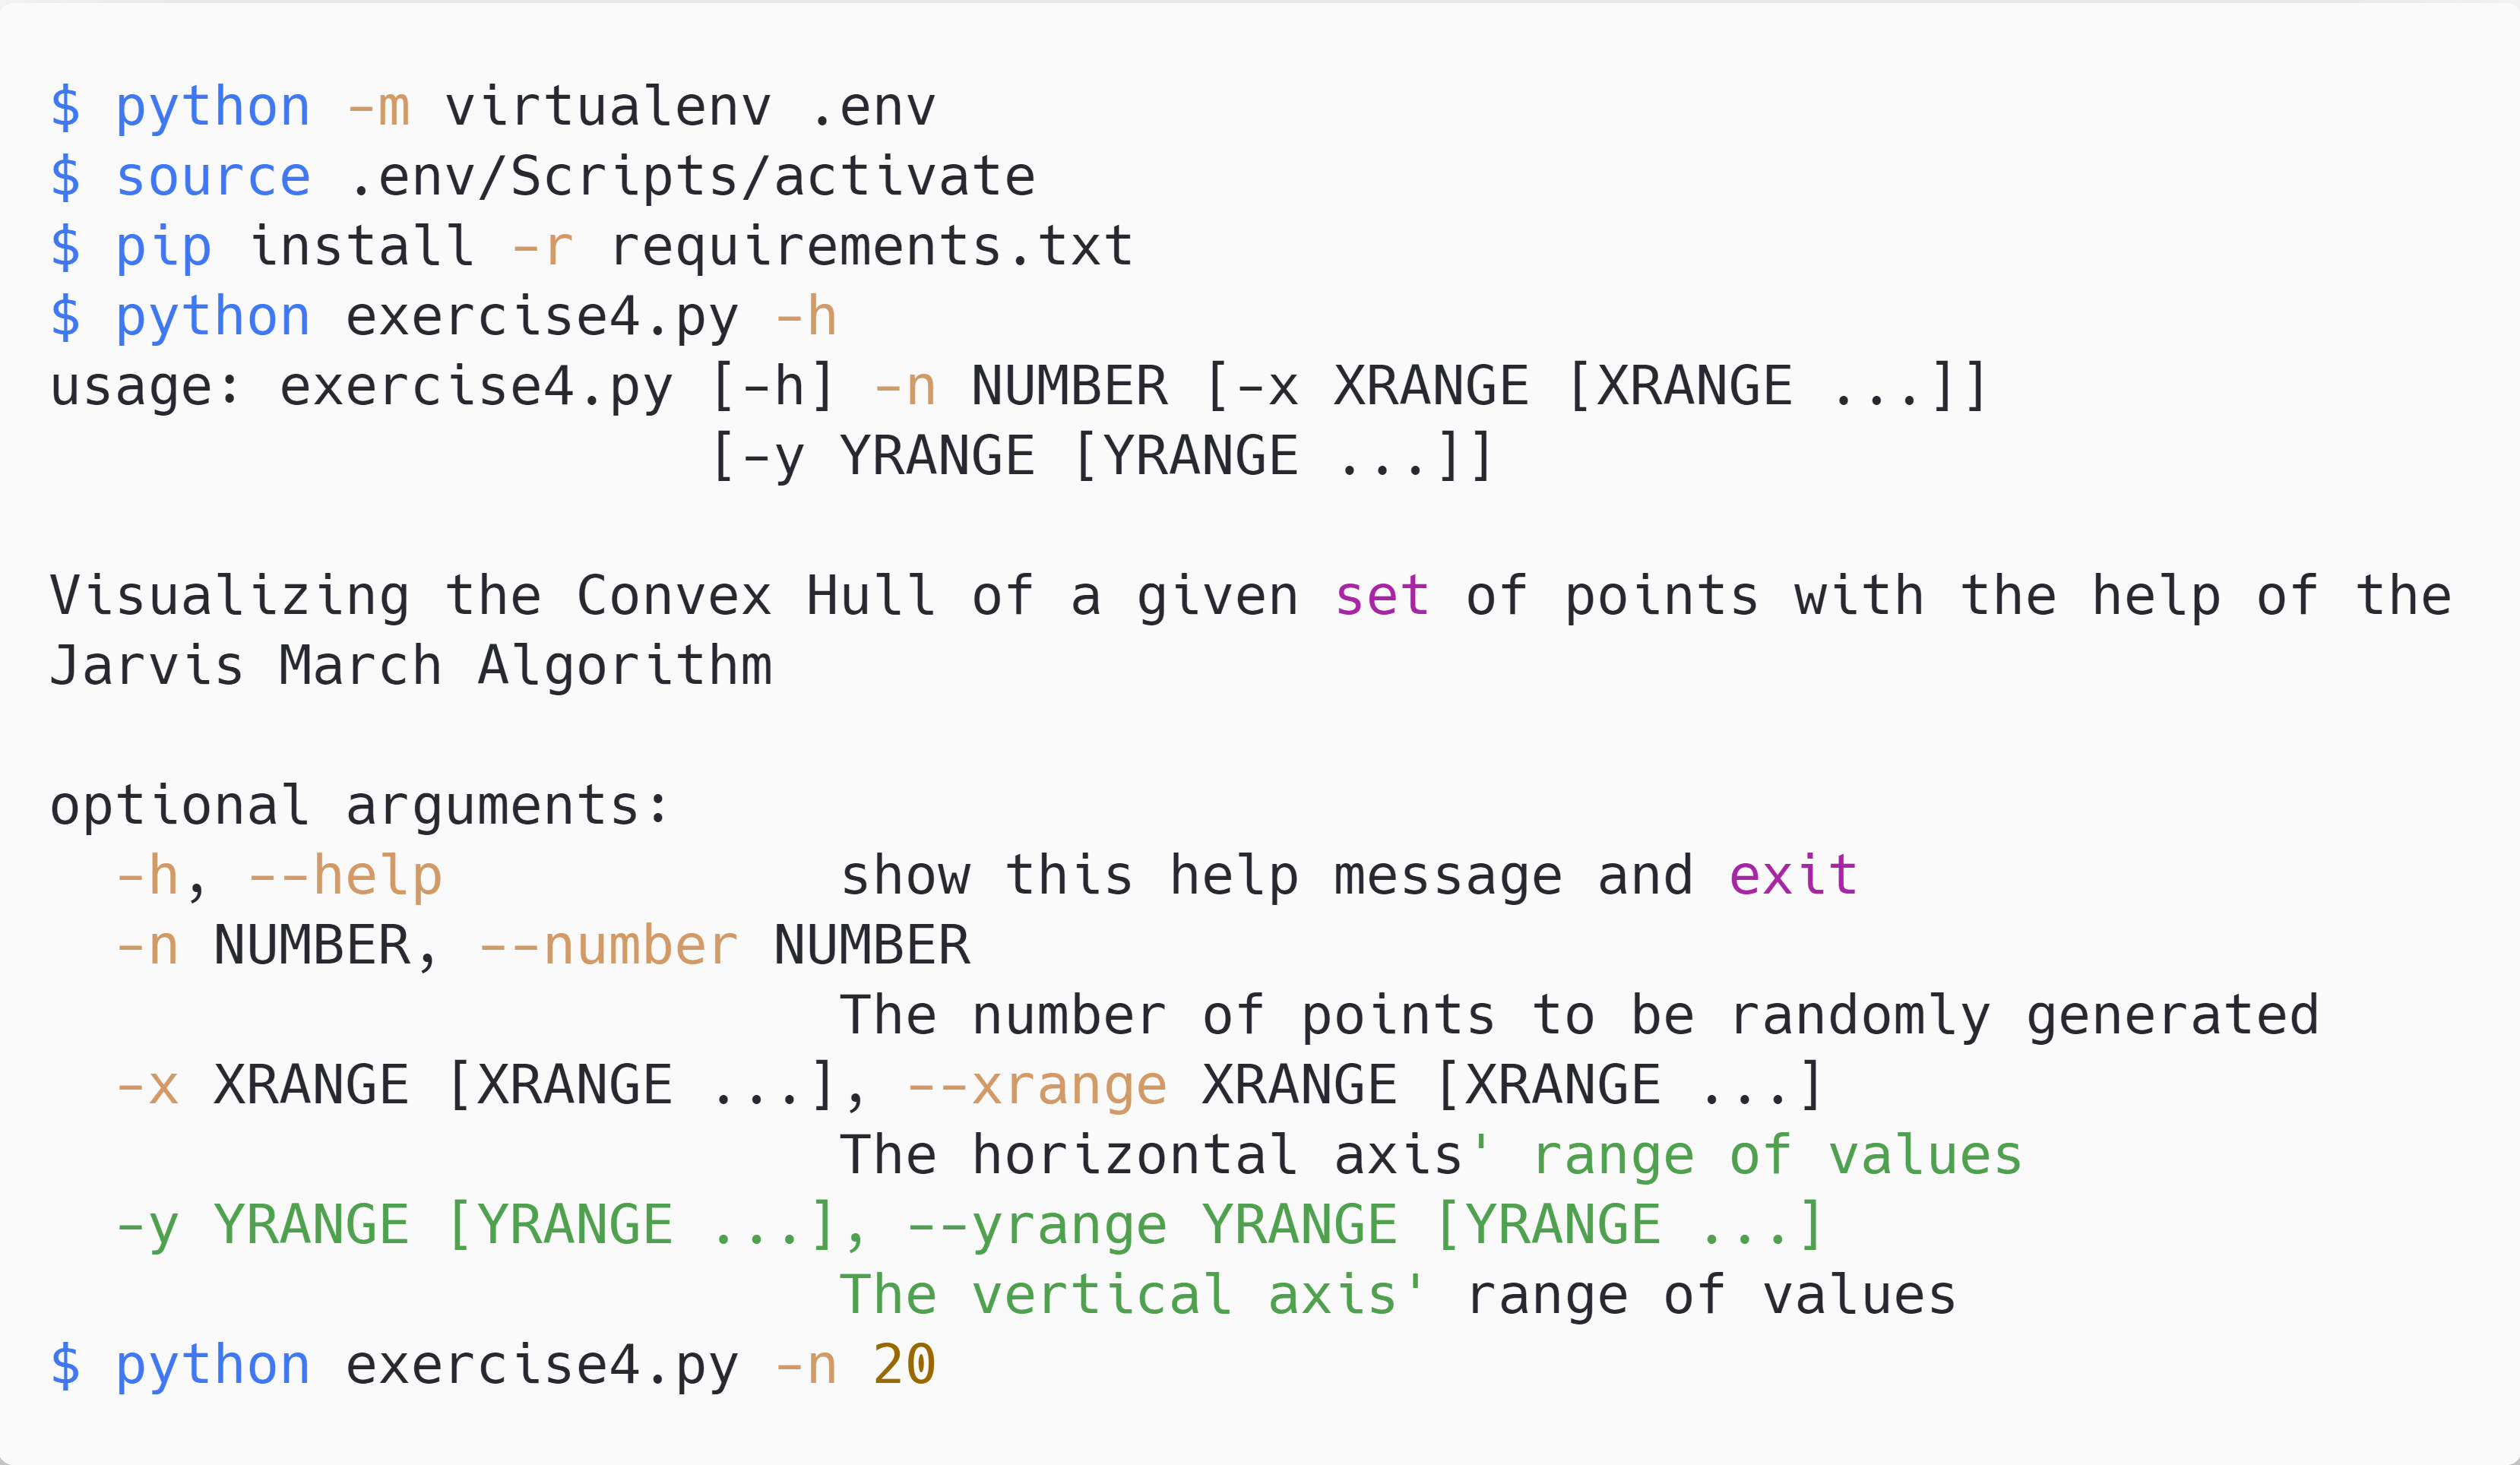
\includegraphics[scale=0.140]{images/gift_wrapping_algorithm.png}
\end{matlab}

\subsubsection*{Example Usage}

\begin{matlab}
    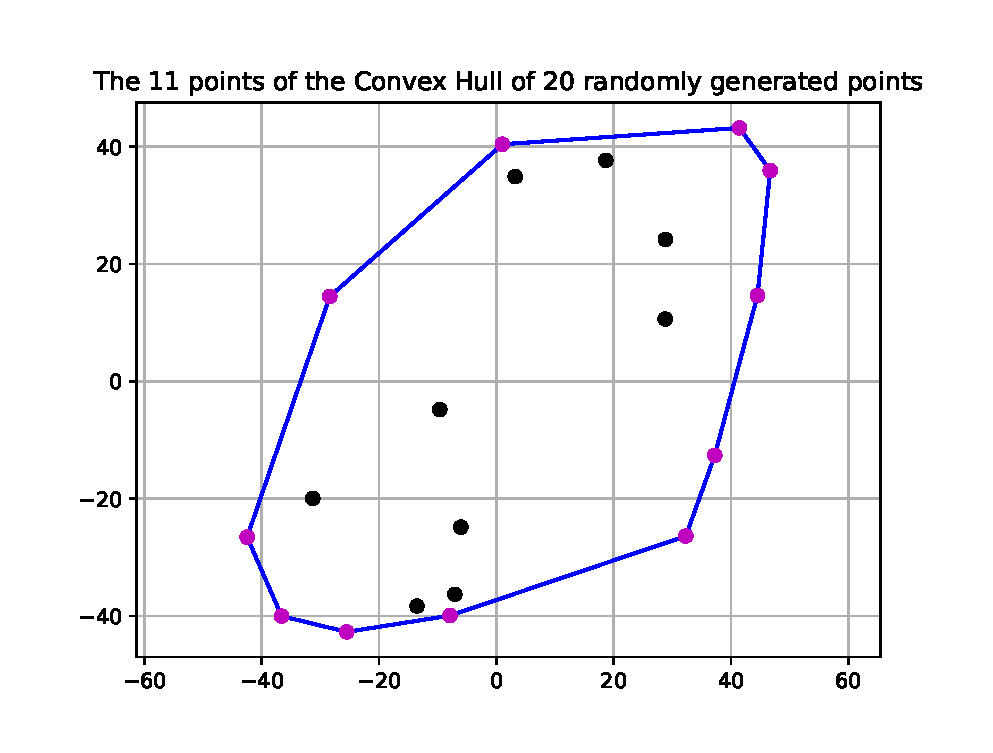
\includegraphics[scale=1]{images/gift_wrapping_algorithm.eps}
\end{matlab}

\pagebreak

\end{document}
